\section{Conclusion and future works}

\begin{frame}{Conclusion}

    We have explored:
    \begin{itemize}
        \item A Knowledge Graph definition incorporating ontologies
        \item A Semantic Web-focused implementation of this Knowledge Graph definition
        \item An OWL Information Retrieval Ontology
        \item Two Knowledge Graph-based Information Retrieval System approaches:
        \begin{itemize}
            \item A real-world use case moving from a text-based to a Knowledge Graph-based Information Retrieval System.
            \item An online OWL reasoning-based Information Retrieval use case.
        \end{itemize}
    \end{itemize}

\end{frame}

\begin{frame}{Future works}

    \begin{itemize}
        \item Knowledge Graph-based Information Retrieval system:
        \begin{itemize}
            \item Expand the Knowledge Graph
            \item Expand the approach to other domains
        \end{itemize}
        \item OWL reasoning-based Information Retrieval system:
        \begin{itemize}
            \item Experiment with a real-world use case at scale
            \item Explore distinguishing between searches with no matching documents and incoherent ones 
        \end{itemize}
        \item Implement an end-to-end Knowledge Graph-Based System architecture use case.
    \end{itemize}

\end{frame}

\begin{frame}{Perspectives: Knowledge Graph}

    \begin{figure} [H]
        \begin{center}
            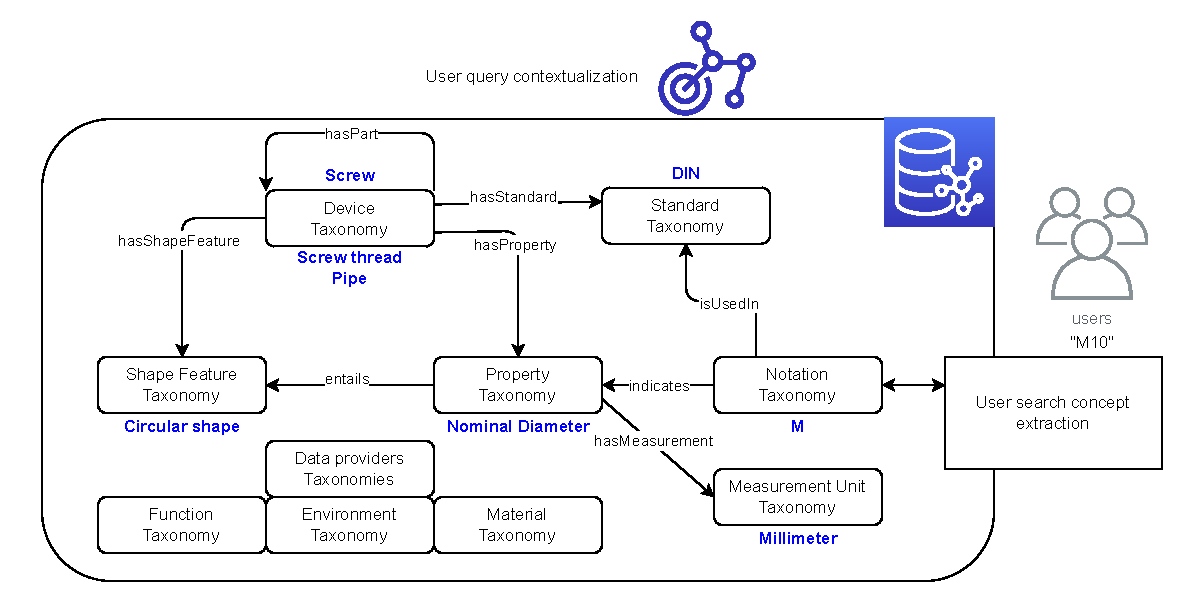
\includegraphics[scale=0.5]{images/semantic_search_example.pdf} 
            \caption{Extended semantic search example.} 
        \end{center}
    \end{figure}

\end{frame}